\documentclass[a4paper,12pt]{scrartcl}
\usepackage[utf8]{inputenc}
\usepackage[UKenglish]{isodate}
\usepackage{csquotes}
\usepackage{graphicx}
\usepackage{wrapfig}
\usepackage{enumitem}
\usepackage{pdflscape}
\usepackage[toc,page]{appendix}
\usepackage{geometry}
\usepackage{hyperref}
\usepackage{cleveref}
\usepackage{listings}
\usepackage{csvsimple}
\usepackage{booktabs}
\usepackage{longtable}
\usepackage{caption}
\usepackage{subcaption}
\usepackage[colorinlistoftodos]{todonotes}
\usepackage[british]{babel}
\usepackage{float}
%\usepackage[margin=1in]{geometry}
\usepackage{listings}
\usepackage{color}
 
\definecolor{codegreen}{rgb}{0,0.6,0}
\definecolor{codegray}{rgb}{0.5,0.5,0.5}
\definecolor{codepurple}{rgb}{0.58,0,0.82}
\definecolor{backcolour}{rgb}{0.95,0.95,0.92}
 
\lstdefinestyle{mystyle}{
	language=PHP,
    backgroundcolor=\color{backcolour},   
    commentstyle=\color{codegray},
    keywordstyle=\color{magenta},
    numberstyle=\tiny\color{codegray},
    stringstyle=\color{codegreen},
    basicstyle=\footnotesize,
    breakatwhitespace=false,         
    breaklines=true,                 
    captionpos=b,                    
    keepspaces=true,                 
    numbers=left,                    
    numbersep=5pt,                  
    showspaces=false,                
    showstringspaces=false,
    showtabs=false,                  
    tabsize=3,
    morekeywords={ new, __halt_compiler, abstract, and, array, as, break, callable, case, catch, class, clone, const, continue, declare, default, die, do, echo, else, elseif, empty, enddeclare, endfor, endforeach, endif, endswitch, endwhile, eval, exit, extends, final, for, foreach, function, global, goto, if, implements, include, include_once, instanceof, insteadof, interface, isset, list, namespace, new, or, print, private, protected, public, require, require_once, return, static, switch, throw, trait, try, unset, use, var, while, xor}
}

\lstset{language=Java,
  showspaces=false,
  showtabs=false,
  breaklines=true,
  showstringspaces=false,
  breakatwhitespace=true,
  commentstyle=\color{pgreen},
  keywordstyle=\color{pblue},
  stringstyle=\color{pred},
  basicstyle=\ttfamily,
  moredelim=[il][\textcolor{pgrey}]{$$},
  moredelim=[is][\textcolor{pgrey}]{\%\%}{\%\%}
}
 
\lstset{style=mystyle}

\graphicspath{ {images/} }
\usepackage[
	backend=biber,
	style=ieee,
	]{biblatex}

\addbibresource{references.bib}

\title{Review of TCP Congestion Control Papers}
\author{Candidate No: 105936}
\date{\today}

\begin{document}
	
	\begin{titlepage}
		\maketitle
	\end{titlepage}
	
	\tableofcontents
	\newpage
	
	\section{Congestion Avoidance and Control\cite{JacobsonCongestAvoidanceControlArticle}}
	{
		This paper was the first to suggest implementing congestion control in TCP. Van Jacobson discovered that the internet was having congestion collapses. This is where throughput would drop to a fraction of what it should be this is because the network would keep dropping packets as there isn't enough bandwidth and the computers would keep resending the failed packets. Jacobson then goes on to outline the congestion control solution which would introduce many features which are still in use such as congestion windows and slow-start.
	}
	\section{Simulation-based Comparisons of Tahoe, Reno, and SACK TCP\cite{FallFloydTahoeRenoSack}}
	{
		This paper outlines how selective acknowledgements could be used to improve the performance of TCP when several are dropped. The paper looks at how Tahoe, Reno, New-Reno and, Sack TCP handle 1,2,3 and, 4 dropped packets. The paper shows that Reno and New-Reno have problems recovering when they have a Fast Retransmit followed by a retransmit timeout and Tahoe struggles with any form of packet loss as it conducts slow-start after every packet loss. The approach of validating the use of Selective acknowledgements are shown in the graphs in the paper\cite{FallFloydTahoeRenoSack} and can be found in \cref{fig:CoparisonOfTCPWith4DroppedPackets}
		\begin{figure}[h]
			\centering
			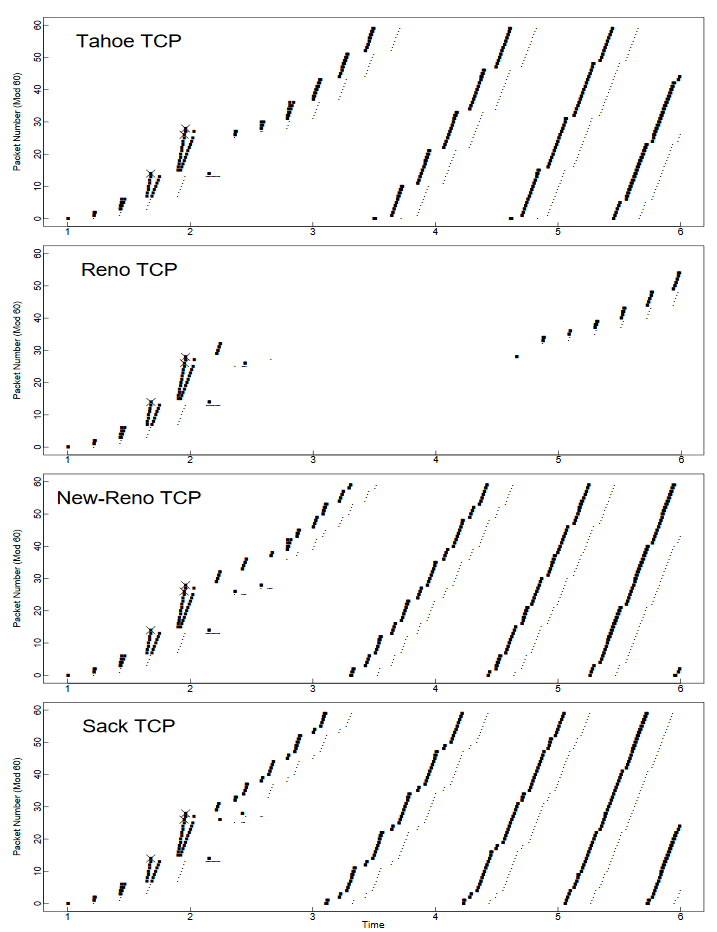
\includegraphics[width=0.75\textwidth]{CoparisonOfTCPWith4DroppedPackets}
			\caption{A Graph showing how the various TCP implementations handle three dropped packets\cite{FallFloydTahoeRenoSack}}
			\label{fig:CoparisonOfTCPWith4DroppedPackets}
		\end{figure}
	}
	\section{CUBIC: a new TCP-friendly high-speed TCP variant\cite{HaRheeXuCubic}}
	{
		This paper proposed a novel new way of implementing BIC(Binary Increase Control) TCP using a cubic function. This provided two benefits, the first is the ability to adjust the width of the curve in the cubic implementation this means that for connections with small round-trip times it wouldn't follow the curve too quickly, a graph showing this can be seen in \cref{fig:BICVsCubicRTT}. The second is implementing the binary increase algorithm is quite computationally expensive, whereas implementing the cubic function would be relatively easy.
		\begin{figure}[h]
			\centering
			\includegraphics[width=0.75\textwidth]{BICVsCubicRTT}
			\caption{An Image showing the difference between CUBIC and BIC with a respect to round-trip times\cite{deawookim2015}}
			\label{fig:BICVsCubicRTT}
		\end{figure}
	}
	\section{Improving Datacenter Performance and Robustness with Multipath TCP\cite{RaiciuBarrePluntkeGreenhalghWischikHandleyMultipathTCPArticle}}
	{
		The paper sets out to answer two questions, What and how large are the benefits to multipath TCP and how to redesign data centre networks to take advantage of multipath TCP. The multiple paths(subflows) are opened on different ports or different IP addresses on the computer if available. Once the subflows are set-up the data to be sent across the multiple paths are striped across the subflows. Each subflow has its own sequence space and congestion window. This allows for load balancing across the network as the paths with more congestion will be used less. The paper also outlines Equally weighted TCP which is an interesting concept to allow for fairness between existing single path TCP flows. This involves dividing the additive increase by the number of subflows.
	}
	\newpage
	\clearpage
	\printbibliography[heading=bibintoc,title=References]
\end{document}
